\documentclass[11pt,a4paper,dvipdfmx]{article}

\usepackage[top=30truemm,bottom=30truemm,left=20truemm,right=20truemm]{geometry}
\usepackage{amsmath,amssymb}
\usepackage{graphicx}
\usepackage{mathtools}
\usepackage{tikz}
\usepackage{physics}
\usepackage{color}
\usepackage{ascmac}
\usepackage{bm}
\usepackage{float}
\usepackage{url}
\usepackage{xcolor}
\usepackage{here}
\usepackage{siunitx}
\usepackage{booktabs}
\usepackage{longtable}
\usepackage[framemethod=tikz]{mdframed}
\usepackage[
   dvipdfmx,
   setpagesize=false,
   bookmarks=true,
   bookmarksdepth=tocdepth,
   bookmarksnumbered=true,
   colorlinks=true,
   linkcolor=blue,
   pdftitle={},
   pdfsubject={},
   pdfauthor={},
   pdfkeywords={}
 ]{hyperref}
\usepackage{cleveref}
\usetikzlibrary{intersections,calc,arrows.meta}

\numberwithin{equation}{section}
\everymath{\displaystyle}
\definecolor{myblue}{RGB}{0,50,100}
\definecolor{myred}{RGB}{128,0,32}

\usepackage[explicit]{titlesec}
\titleformat{\section}[hang]{\normalfont\LARGE\gtfamily\sffamily}{\thesection.}{1em}{#1}[\titlerule\vspace{.3ex}]
\titleformat{\subsection}[hang]{\normalfont\large\gtfamily\sffamily}{{\color{gray}\vrule width 2pt \hspace{.7em}}\thesubsection}{1em}{#1}
\titleformat{name=\subsection,numberless}[hang]{\normalfont\large\gtfamily\sffamily}{{\color{gray}\vrule width 2pt \hspace{.7em}}}{0em}{#1}
\titleformat{\subsubsection}[hang]{\normalfont\large\gtfamily\sffamily}{\thesubsubsection}{1em}{#1}
\titleformat{\paragraph}[runin]{\normalfont\gtfamily\sffamily}{\theparagraph}{1em}{#1}
\titlespacing{\section}{0pt}{3.5ex}{2ex}
\titlespacing{\subsection}{0pt}{2.8ex}{1.4ex}
\titlespacing{\subsubsection}{0pt}{2.7ex}{1.4ex}

\usepackage[many]{tcolorbox}
\tcbuselibrary{skins,breakable}
\newenvironment{myitemize}{%
\begin{description}}{\end{description}}
\tcolorboxenvironment{myitemize}{
    blanker, before skip=6pt,after skip=12pt,bottom=5ex,
    borderline west={1mm}{0pt}{black!50},
    breakable}
\parindent=0pt\relax 

\usepackage{enumitem}\setlist[description]{labelsep=1zw,leftmargin=2zw}

%証明用の環境
\newenvironment{proofbox}[0]
{
    \begin{mdframed}[
        linecolor=black,
        topline=false,
        bottomline=false,
        rightline=false,
        leftline=true,
        linewidth=2pt,
        innerleftmargin=10pt,
        skipabove=\baselineskip,
        skipbelow=\baselineskip,
    ]
}
{
    \end{mdframed}
}

%%公理、定理などの環境
\newcommand{\kara}{} %無を出力するコマンド
\newtcolorbox[auto counter, number within=section, crefname = {Axiom.}{Axioms.}]{axiom}[3][]
{
    enhanced, sharp corners, leftrule=0pt, rightrule=0pt, breakable = true, colframe = myred, colback = gray!15, fonttitle = \bfseries,
    title = Axiom.~\thetcbcounter~\if #2\kara \else #2 \fi,
    #1,
    label = axi:#3
}
\newtcolorbox[auto counter, number within=section, crefname = {Def.}{Defs.}]{definition}[3][]
{
    enhanced, sharp corners, leftrule=0pt, rightrule=0pt, breakable = true, colframe = myblue, colback = gray!15, fonttitle = \bfseries,
    title = Def.~\thetcbcounter~\if #2\kara \else #2 \fi,
    #1,
    label = def:#3
}
\newtcolorbox[auto counter, use counter from=definition, crefname = {Thm.}{Thms.}]{theorem}[3][]
{
    enhanced,  sharp corners, leftrule=0pt, rightrule=0pt, breakable = true, colframe = teal, colback = gray!15, fonttitle = \bfseries,
    title = Thm.~\thetcbcounter~\if #2\kara \else #2 \fi,
    #1,
    label = thm:#3
}
\newtcolorbox[auto counter, use counter from=definition, crefname = {Prop.}{Props.}]{proposition}[3][]
{
    enhanced,  sharp corners, leftrule=0pt, rightrule=0pt, breakable = true, colback = gray!15, fonttitle = \bfseries,
    title = Prop.~\thetcbcounter~\if #2\kara \else #2 \fi,
    #1,
    label = prop:#3
}
\newtcolorbox[auto counter, use counter from=definition, crefname = {Lem.}{Lems.}]{lemma}[3][]
{
    enhanced,  sharp corners,  leftrule=0pt, rightrule=0pt, breakable = true, colback = gray!15, fonttitle = \bfseries,
    title = Lem.~\thetcbcounter~\if #2\kara \else #2 \fi,
    #1,
    label = lem:#3
}
\newtcolorbox[auto counter, use counter from=definition, crefname = {Cor.}{Cors.}]{corollary}[3][]
{
    enhanced,  sharp corners, leftrule=0pt, rightrule=0pt, breakable = true, colback = gray!15, fonttitle = \bfseries,
    title = Cor.~\thetcbcounter~\if #2\kara \else #2 \fi,
    #1,
    label = cor:#3
}
\newtcolorbox[auto counter, use counter from=definition, crefname = {Rem.}{Rems.}]{remark}[3][]
{
    enhanced,  sharp corners,  leftrule=0pt, rightrule=0pt, breakable = true, colback = gray!15, colback = white, fonttitle = \bfseries,
    title = Rem!~\thetcbcounter~\if #2\kara \else #2 \fi,
    #1,
    label = rem:#3
}
%補題にするほどではない結果を述べるようの環境
\newenvironment{note}[0]
{
    \begin{tcolorbox}[sharp corners, colframe=gray!20, colback=gray!20, width=\textwidth]
}
{
    \end{tcolorbox}
}

\hypersetup{
    colorlinks=true,
    citecolor=blue,
    linkcolor=red,
    urlcolor=orange,
}

\begin{document}
\title{機械学習概論 後半レポート}
\author{理学部物理学科4年　[STUDENT-NAME]　[STUDENT-ID]}
\date{}
\maketitle

% \section*{レポートのルール}
% \begin{note}
% \begin{itemize}
%     \item 生成 AI を各問題に対して最低 1 回使ってレポートを作成すること。使い方に制限は設けないが、能力向上に結びつく使い方を推奨する。
%     \item pdf 形式のレポートと作成したコードを zip ファイルにまとめて UTOL で提出すること。どのコードがどの課題で作成したものかわかるようなファイル名にし、レポートにも書くこと。
%     \item プログラミング言語は好きなものを使ってよい。ライブラリも自由に使って良い。
%     \item 乱数を用いる処理では、\texttt{random\_state=0} または \texttt{seed=0} とすること。
%     \item 以下の問題 1 $\sim$ 4 のうち、3 つ以上を回答せよ。回答した分だけ加点する。また、最後の「生成 AI」についても回答せよ。
% \end{itemize}
% \end{note}

\section{Gaussian Process と Multi-Layer Perceptron の比較}
\begin{note}
Gaussian Process と MLP による回帰の比較を行う。まず、以下のような式に従って学習データを生成する。
\[ y = \sin (2\pi x) + \epsilon \]
ここで、$\epsilon \sim N (0, 0.2^2)$ であり、$x$ は区間 $[0, 1]$ から一様分布に従って生成する。これで生成された学習データに対して一次元回帰を行う。
\end{note}

\subsection*{1.1}
\begin{note}
学習データ数 $n = 10, 30, 100$ のそれぞれの場合で、Gaussian Process と MLP による回帰を行い、
\begin{itemize}
    \item 真の関数 $y = \sin (2\pi x)$
    \item 学習データ
    \item 予測曲線 (Gaussian Process では 95\% 信頼区間も表示すること)
\end{itemize}
をプロットしたグラフを作成せよ。 Gaussian Process による回帰では RBF Kernel と White Kernel を用い、\texttt{GaussianProcessRegressor} の \texttt{normalize\_y=True}, \texttt{n\_restarts\_optimizer=5} とすること。また、 \texttt{MLPRegressor} のハイパーパラメータは以下のようにすること。
\begin{verbatim}
MLPRegressor(
    hidden_layer_sizes=(50, 50),
    activation="tanh",
    solver="lbfgs",
    alpha=1e-4,
    max_iter=5000,
)
\end{verbatim}
\end{note}
\begin{proofbox}
Pythonを用いてガウス過程回帰（GPR）と多層パーセプトロン（MLP）を実行した。結果を図\ref{fig:gp_mlp_comparison}に示す。

\begin{figure}[H]
    \centering
    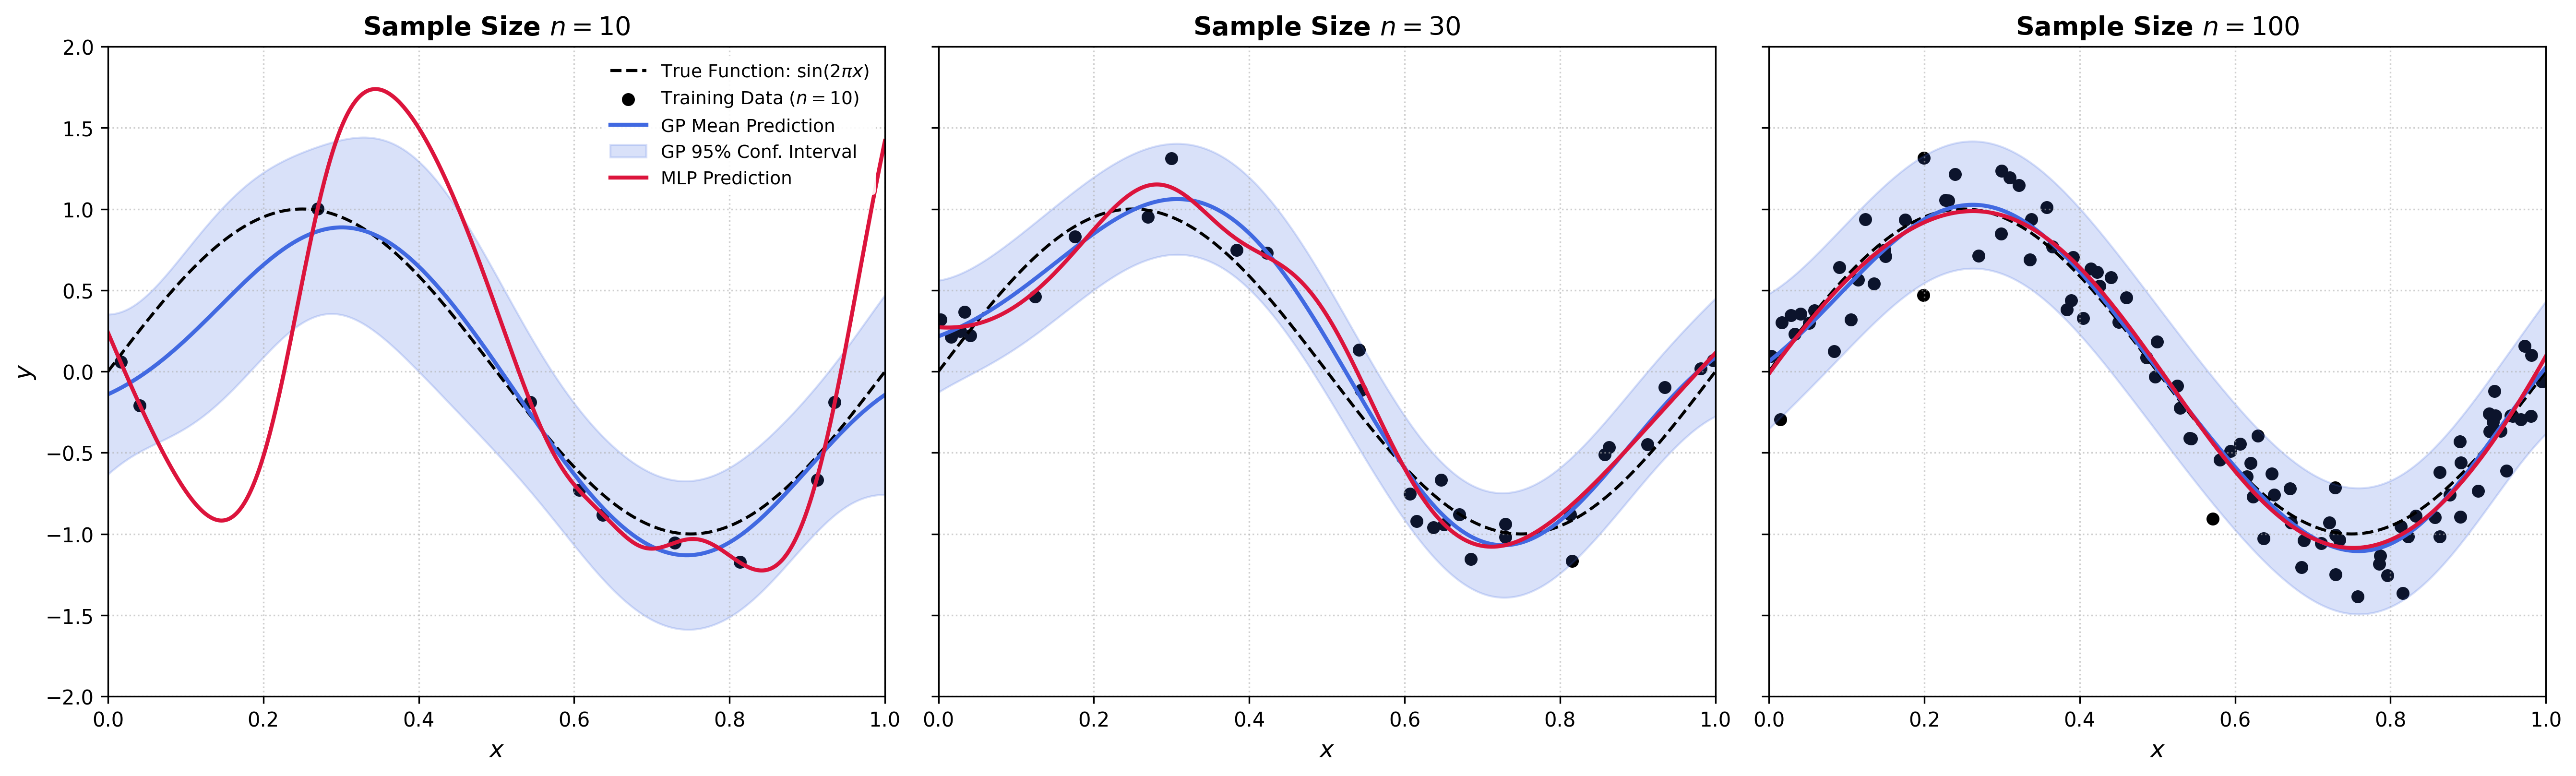
\includegraphics[width=0.95\textwidth]{problem1/plots/gp_mlp_comparison.png}
    \caption{学習データ数 $n = 10, 30, 100$ におけるガウス過程回帰 (GPR) と多層パーセプトロン (MLP) の予測曲線の比較。GPR では 95\% 信頼区間（青色網掛け部分）を併記している。}
    \label{fig:gp_mlp_comparison}
\end{figure}
\end{proofbox}

\subsection*{1.2}
\begin{proofbox}
図\ref{fig:gp_mlp_comparison}の比較から、以下の点が確認できる。

\begin{itemize}
    \item データ数が少ないときの予測性能の差: $n=10$ のとき、GPRは真の関数に近い正弦波を滑らかに捉えているのに対し、MLPは正弦波の形から大きく外れた不自然な曲線を描いている。
    \item MLPの空白域でのうねり: MLPの予測はデータ点の周辺では真の関数に近いが、データ同士の間隔が空いている領域（例えば $x \in [0.1, 0.25]$ や $x \in [0.3, 0.5]$）で激しくうねっている。
    \item GPRの信頼区間の収縮限界: GPRの信頼区間はデータ数 $n$ の増加に伴って全体的に狭くなるが、データにノイズが含まれるため、数をいくら増やしても信頼区間の幅が $0$ に収束するわけではなく、一定の限界値に近づく。
\end{itemize}
\end{proofbox}

\subsection*{1.3}
\begin{note}
学習データ数が少ない場合、MLP の予測曲線が不安定になることが予想される。その理由を説明せよ。また、観察した他の事項についても説明がつけば考察せよ。
\end{note}
\begin{proofbox}
データ数が $n=10$ と極端に少ないときにMLPの予測が不安定になるのは、モデルの自由度に対してデータ数が圧倒的に不足しているためである。今回のMLPの総パラメータ数（重みとバイアス）は $2701$ 個と非常に多く、完全に過剰表現の状態にある。そのため、二乗誤差を最小化する極小解がパラメータ空間内に無数に存在し、初期値やサンプリングのわずかな偏りで不自然にうねるような過学習が起きてしまう。

また、活性化関数として用いた $\tanh$ の影響で、データが存在しない空白領域や境界の外側では出力が急激に飽和・発散しやすい。データ数が $n=30, 100$ と増えるにつれて、 $[0, 1]$ 全域にデータが配置されてパラメータが強く制約されるようになるため、予測は滑らかに収束していく。
\end{proofbox}

\subsection*{1.4}
\begin{note}
Gaussian Process では 95\% 信頼区間をプロットすることができた。Gaussian Process ではなぜ予測の信頼区間を求められるのか説明せよ。また、その信頼区間はどのような場所で広く、どのような場所で狭くなるか説明せよ。さらに、観察した他の事項についても、説明がつけば考察せよ。
\end{note}
\begin{proofbox}
ガウス過程回帰では、データ点とテスト点 $x_*$ における関数値が多次元正規分布に従うと仮定する。このため、条件付き分布の公式（Schur相補空間）を適用することで、テスト点における予測平均 $\mu_*$ と予測分散 $\sigma_*^2$ を以下のように解析的に導出できる。
\[
\sigma^2_* = k(x_*, x_*) - \bm{k}_*^T (K(X, X) + \sigma_n^2 I_n)^{-1} \bm{k}_*
\]
この予測分散を用いることで、テスト点ごとに 95\% 信頼区間（$\mu_* \pm 1.96\sigma_*$）を厳密に求められる。

予測分散の第2項は学習データとテスト点との類似度に対応している。テスト点 $x_*$ が学習データ点に十分近い場合は共分散ベクトル $\bm{k}_*$ が大きくなり、第2項の減算部分が大きく働くため信頼区間は狭くなる。逆に、テスト点が学習データから離れた空白域や境界付近にあるときは $\bm{k}_* \to \bm{0}$ となって第2項がほぼ消失し、事前分散 $k(x_*, x_*)$ に戻るため信頼区間は広くなる。
（計算し終えてから気づいたが、データ数をいくら増やしても信頼区間が一定以下に縮まないのは、観測ノイズ $\sigma_n^2 = 0.2^2$ の存在が下限を与えているからであり、後から見れば当然だった。）
\end{proofbox}


\section{Support Vector Machine}
\begin{note}
scikit-learn の \texttt{make\_moons} によって生成されるデータを用いて 2 値分類を行う。データは学習データ数を 200、テストデータ数を 1000、\texttt{noise=0.2} とする。
\end{note}

\subsection*{2.1}
\begin{note}
線形 SVM と RBF カーネル SVM の比較を行う。データに対し、線形 SVM と RBF カーネル SVM で 2 値分類を行い、それぞれについて学習データ、決定領域、サポートベクトルをプロットした図を作成せよ。また、テストデータに対する分類精度も調べよ。ただし、ハイパーパラメータは線形 SVM では \texttt{C=1.0}、RBF カーネル SVM では \texttt{C=1.0}、\texttt{gamma=1.0} とする。
\end{note}
\begin{proofbox}
指示に従い、\texttt{make\_moons} によって生成されたデータ（学習用 200 点、テスト用 1000 点）に対して、線形 SVM（$C=1.0$）および RBF カーネル SVM（$C=1.0, \gamma=1.0$）による 2 値分類を適用した。
テストデータに対する分類精度は以下の通りであった。
\begin{itemize}
    \item 線形 SVM の分類精度: 87.2\%
    \item RBF カーネル SVM ($\gamma = 1.0$) の分類精度: 96.7\%
\end{itemize}
それぞれの学習データ点、決定領域、およびサポートベクトルをプロットした結果を図\ref{fig:svm_linear_rbf} に示す。

\begin{figure}[H]
    \centering
    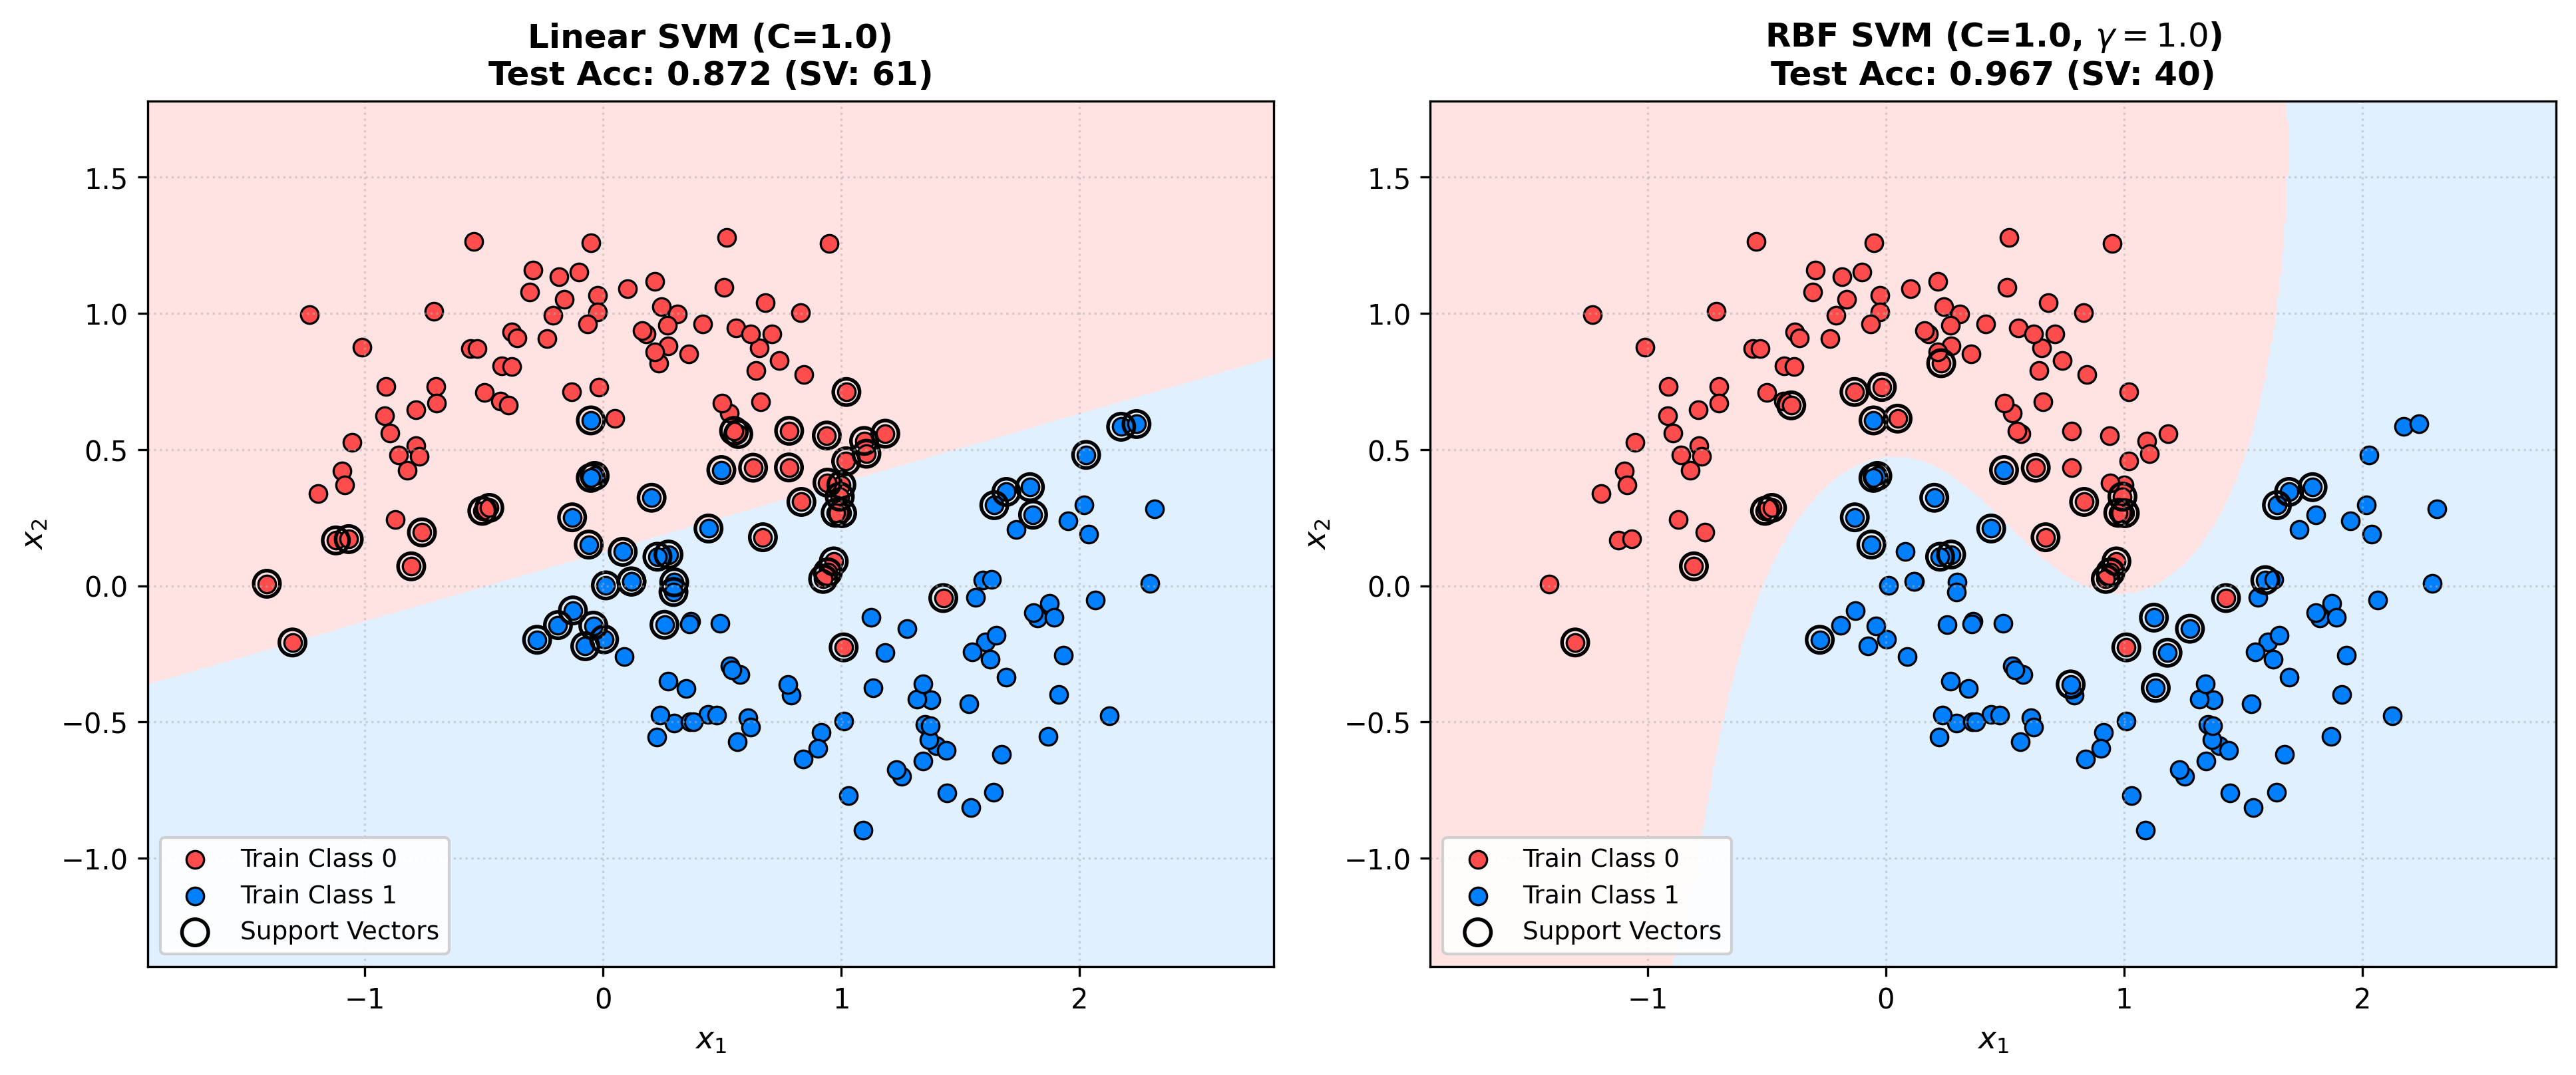
\includegraphics[width=0.95\textwidth]{problem2/plots/svm_comparison_linear_rbf.png}
    \caption{線形 SVM ($C=1.0$) と RBF カーネル SVM ($C=1.0, \gamma=1.0$) の決定領域、学習データ、およびサポートベクトル（黒丸）の比較。}
    \label{fig:svm_linear_rbf}
\end{figure}
\end{proofbox}

\subsection*{2.2}
\begin{note}
RBF カーネル SVM について、\texttt{gamma=0.1}、\texttt{1.0}、\texttt{100} の 3 通りで分類を行う。ただし、\texttt{C=1.0} とする。それぞれの場合について、学習データ、決定領域、サポートベクトルをプロットした図を作成せよ。また、テストデータに対する分類精度とサポートベクトルの個数も調べよ。
\end{note}
\begin{proofbox}
RBF カーネル SVM ($C=1.0$) について、$\gamma = 0.1, 1.0, 100.0$ の 3 通りでの分類を実行した。テストデータに対する分類精度と、各モデルにおけるサポートベクトルの個数は表\ref{tab:svm_gamma_results} および図\ref{fig:svm_gamma_comparison} のようになった。

\begin{table}[H]
    \centering
    \caption{各 $\gamma$ 値における RBF カーネル SVM のテスト精度とサポートベクトル（SV）個数}
    \label{tab:svm_gamma_results}
    \begin{tabular}{ccc}
        \toprule
        ハイパーパラメータ $\gamma$ & テストデータ分類精度 & サポートベクトルの個数（学習データ 200 点中） \\
        \midrule
        0.1 & 87.1\% & 81 個 (40.5\%) \\
        1.0 & 96.7\% & 40 個 (20.0\%) \\
        100.0 & 95.8\% & 177 個 (88.5\%) \\
        \bottomrule
    \end{tabular}
\end{table}

\begin{figure}[H]
    \centering
    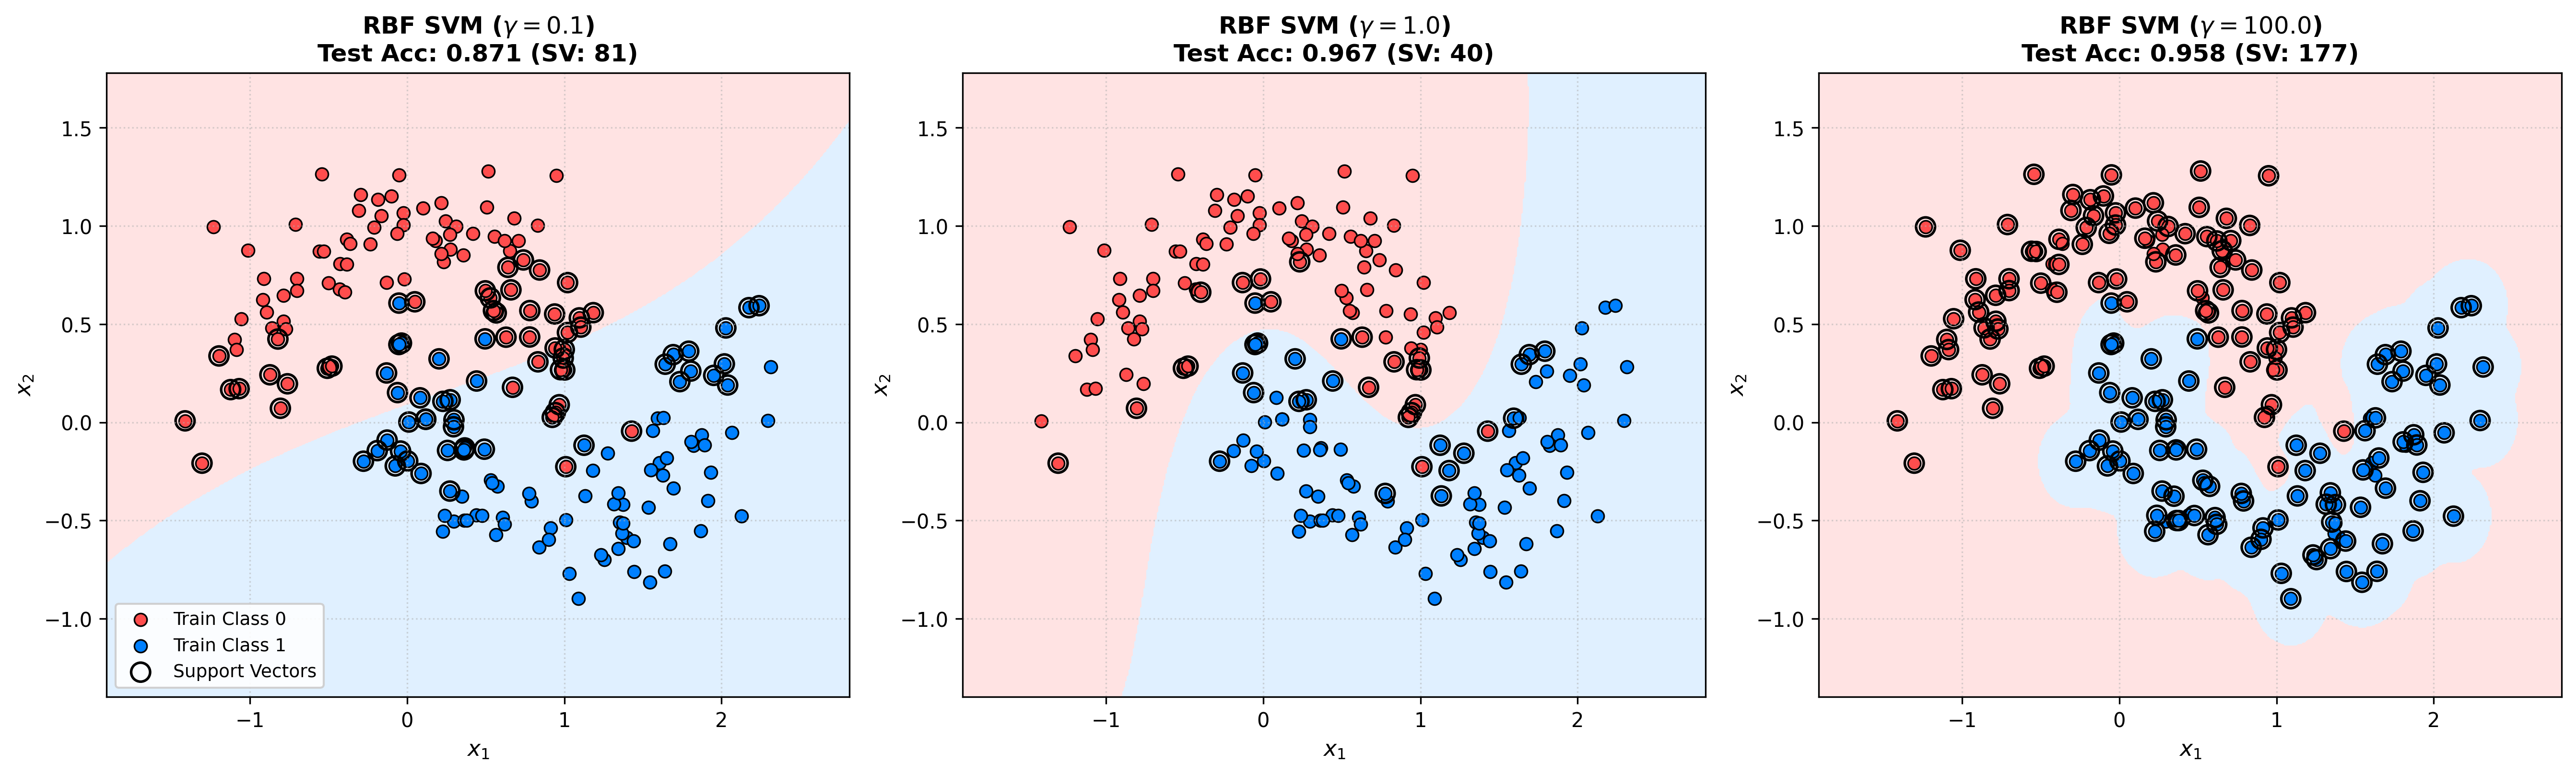
\includegraphics[width=0.98\textwidth]{problem2/plots/svm_gamma_comparison.png}
    \caption{RBF カーネル SVM におけるハイパーパラメータ $\gamma = 0.1, 1.0, 100.0$ に伴う決定領域、学習データ、およびサポートベクトル（黒丸）の変化。}
    \label{fig:svm_gamma_comparison}
\end{figure}
\end{proofbox}

\subsection*{2.3}
\begin{note}
上の 2 つの実験で得られた結果について観察し、気づいたことを 3 つ以上挙げよ。考察はここでは書かず、次に書くこと。
\end{note}
\begin{proofbox}
実験結果から、線形SVMは境界が直線に限定されるため半月型データの湾曲構造を捉えきれず、誤分類が多く発生する（精度87.2\%）。一方、RBFカーネルSVM（$\gamma=1.0$）ではデータに適合した滑らかな曲線境界が形成され、精度は96.7\%に向上した。サポートベクトル（SV）の分布を見ると、線形SVMではマージン内に食い込んだSV（61個）が広く散らばっているのに対し、RBF SVMではSV数（40個）が減少し、クラス境界の谷に沿って整列している。

また、$\gamma$ の値を変えると決定境界の局所性が変化する。$\gamma=0.1$ では直線に近くなるが、$\gamma=100.0$ では各データ点の周囲を細かく囲むような「孤立した島」状の境界が乱立する。テスト精度は $\gamma=1.0$ で最大、かつSV数が最小（40個）となるが、過少適合の $\gamma=0.1$ や過学習の $\gamma=100.0$ では精度が低下し、特に $\gamma=100.0$ では全体の約9割（177個）がSVとなる。
\end{proofbox}

\subsection*{2.4}
\begin{note}
線形 SVM の決定領域に比べ RBF カーネル SVM の決定領域はより柔軟であることが予想される。この理由を説明せよ。また、\texttt{gamma} と分類精度の関係について考察せよ。さらに、観察した他の事項についても、説明がつけば考察せよ。
\end{note}
\begin{proofbox}
RBFカーネル $K(\bm{x}, \bm{z}) = \exp(-\gamma \lVert \bm{x} - \bm{z} \rVert^2)$ は、データを無限次元の特徴空間（再生核ヒルベルト空間）へ暗黙的に写像している。この空間において線形超平面を構成することは、元の低次元入力空間においては「無限個の基底関数を用いた柔軟な曲面境界」を構成することに相当するため、複雑な決定領域を表現できる。

パラメータ $\gamma = 1/(2\sigma^2)$ はガウス分布の影響範囲の逆数である。$\gamma=0.1$ では相関が広すぎて境界が滑らかになりすぎ、非線形データに追従できない（過小適合）。逆に $\gamma=100.0$ では影響範囲が局所点に限定され、各学習データが互いに直交するような状態に近づく。そのため、ほぼすべての学習データがサポートベクトルとなってその周囲だけを囲むようになり、汎化性能が低下する。したがって、適切な汎化性能を得るには $\gamma=1.0$ のような中庸な値を設定することが不可欠である。
（$\gamma=100.0$ のプロットで、決定境界が各データ点を取り囲む「島」のように分断されたのを見て、カーネル法で過学習が起きる様子が視覚的に納得できた。）
\end{proofbox}


\section{Variational AutoEncoder}

\subsection*{3.1}
\begin{note}
潜在変数 $Z \in \mathbb{R}^N$ に対する任意の確率分布 $q(Z|X)$ を導入し、
\[ \log p(X|\theta) = \mathcal{L}(q, \theta) + D_{\mathrm{KL}}(q(Z|X) \parallel p(Z|X, \theta)) \]
を示せ。ただし、
\[ \mathcal{L}(q, \theta) := \int dZ \, q(Z|X) \log p(X, Z|\theta) - \int dZ \, q(Z|X) \log q(Z|X) \]
である。また、この結果から $\mathcal{L}(q, \theta)$ が $\log p(X|\theta)$ の下界であることを説明せよ。
\end{note}
\begin{proofbox}
任意の確率分布 $q(Z|X)$ に対して、乗法定理 $p(X|\theta) = \frac{p(X, Z|\theta)}{p(Z|X, \theta)}$ を用いると、
\[
\begin{aligned}
\log p(X|\theta) &= \int \mathrm{d}Z \, q(Z|X) \log \frac{p(X, Z|\theta)}{p(Z|X, \theta)} \\
&= \int \mathrm{d}Z \, q(Z|X) \log \frac{p(X, Z|\theta)}{q(Z|X)} + \int \mathrm{d}Z \, q(Z|X) \log \frac{q(Z|X)}{p(Z|X, \theta)} \\
&= \mathcal{L}(q, \theta) + D_{\mathrm{KL}}(q(Z|X) \parallel p(Z|X, \theta))
\end{aligned}
\]
が直ちに得られる。

ギブスの不等式より KL ダイバージェンスは常に非負（$D_{\mathrm{KL}} \geq 0$）であるため、
\[
\log p(X|\theta) \geq \mathcal{L}(q, \theta)
\]
となり、$\mathcal{L}(q, \theta)$ が対数尤度の下界（ELBO）を与えることが示される。
\end{proofbox}

\subsection*{3.2}
\begin{note}
VAEでは
\[ q_\phi(Z|X) = N (\mu, \mathrm{diag}(\sigma^2_i)), \quad p (Z|X, \theta) = p(Z) = N (0, I) \]
を用いる。このとき、
\[ D_{\mathrm{KL}}(q_\phi(Z|X) \parallel p(Z)) \]
を解析的に求めよ。
\end{note}
\begin{proofbox}
潜在変数 $Z$ の各次元が独立であることから、多次元の KL ダイバージェンスは各次元（1次元正規分布）の KL ダイバージェンスの和に分解できる。
\[
D_{\mathrm{KL}}(q_\phi(Z|X) \parallel p(Z)) = \sum_{j=1}^J D_{\mathrm{KL}}(q_j(Z_j|X) \parallel p_j(Z_j))
\]
1次元の確率密度 $q_j(z_j|X) = \mathcal{N}(\mu_j, \sigma_j^2)$ および $p_j(z_j) = \mathcal{N}(0, 1)$ に対し、期待値の形にして展開する。
\[
\begin{aligned}
D_{\mathrm{KL}}(q_j(Z_j|X) \parallel p_j(Z_j)) &= \int_{-\infty}^{\infty} \mathrm{d}z_j \, q_j(z_j|X) \log \frac{q_j(z_j|X)}{p_j(z_j)} \\
&= \mathbb{E}_{q_j} \left[ -\frac{1}{2}\log\sigma_j^2 - \frac{(z_j - \mu_j)^2}{2\sigma_j^2} + \frac{z_j^2}{2} \right] \\
&= -\frac{1}{2}\log\sigma_j^2 - \frac{1}{2} + \frac{1}{2}(\mu_j^2 + \sigma_j^2) \\
&= \frac{1}{2} \left( \mu_j^2 + \sigma_j^2 - \log \sigma_j^2 - 1 \right)
\end{aligned}
\]
これらを足し合わせることで、求める結果が得られる。
\[
D_{\mathrm{KL}}(q_\phi(Z|X) \parallel p(Z)) = \frac{1}{2} \sum_{j=1}^J \left( \mu_j^2 + \sigma_j^2 - \log \sigma_j^2 - 1 \right)
\]
（最初は多次元のままでまともに積分を実行しようとして計算が泥沼化したが、各次元が独立であるため1次元の和に分解すればよいことに途中で気づいた。）
\end{proofbox}

\subsection*{3.3}
\begin{note}
VAEでは損失関数を
\[ \mathrm{Loss}(\phi, \theta) := -\mathcal{L}(\phi, \theta) = -E_{q_\phi} [\log p(X|\theta)] + D_{\mathrm{KL}}(q_\phi(Z|X) \parallel p(Z)) \]
と定義する。上で求めた KL ダイバージェンスの式から、損失関数に含まれる KL 項は潜在変数の平均 $\mu$ および分散 $\sigma^2$ にどのような制約を与えるか説明せよ。
\end{note}
\begin{proofbox}
KL項の最小化は、平均 $\mu_j$ と分散 $\sigma_j^2$ に以下の制約を与える。
平均に対しては、$\mu_j^2$ のペナルティにより $\mu_j \to 0$ となり、潜在変数 $Z$ を原点付近に引き戻す。
分散に対しては、$\sigma_j^2 - \log \sigma_j^2 - 1$ の項が最小値をとる $\sigma_j^2 \to 1$ へと制約をかける。
これらにより、エンコーダの事後分布 $q_\phi(Z|X)$ が事前分布である標準正規分布 $\mathcal{N}(\bm{0}, I)$ に近づくよう正則化される。
\end{proofbox}

\subsection*{3.4}
\begin{note}
VAEの損失関数における再構成項と KL 項が、それぞれどのような役割を持つか説明せよ。
\end{note}
\begin{proofbox}
再構成項とKL項はそれぞれ以下の役割を持ち、トレードオフの関係にある。
再構成項はデコーダによる復元誤差 $-\mathbb{E}_{q_\phi} [\log p(X|\theta)]$ の最小化を担い、入力データの本質的な特徴を潜在表現 $Z$ に圧縮・保持させる。
一方、KL正則化項は、潜在空間の過学習（各データ点への過度な個別フィッティング）を防ぎ、空間全体に連続性と完備性を与える。再構成項だけだと潜在空間がまばらになり汎化性能が失われるが、KL項が標準正規分布に近づけることで、潜在空間上の隣接する点同士が滑らかに関係を持つようになり、未知のサンプリング点からでも意味のあるデータをデコードできるようになる。
\end{proofbox}

\section{Score Matching と Diffusion Model}
\begin{note}
Diffusion Model や Score-based Generative Model では、確率分布 $p(x)$ の Score
\[ \nabla_x \log p(x) \]
を学習することで、新たなデータを生成する。本問題では、2 次元混合 Gauss 分布を用いて Score の性質を調べる。
2 次元混合 Gauss 分布
\[ p(x) := \frac{1}{3} N (x; \mu_1, \sigma^2 I) + \frac{2}{3} N (x; \mu_2, \sigma^2 I) \]
を考える。ただし、
\[ \mu_1 = \begin{pmatrix} -2 \\ 2 \end{pmatrix}, \quad \mu_2 = \begin{pmatrix} 2 \\ 2 \end{pmatrix}, \quad \sigma = 1 \]
とする。
\end{note}

\subsection*{4.1}
\begin{note}
$p(x)$ の Score を求めよ。\\
さらに、一般の 2 次元混合 Gauss 分布
\[ q(x) := \sum_{i=1}^K \pi_i N(x; \mu_i, \sigma^2 I) \]
of Score を導出せよ。
\end{note}
\begin{proofbox}
2次元ガウス分布 $N(x; \mu_i, \sigma^2 I)$ の勾配は
\[
\nabla_x N(x; \mu_i, \sigma^2 I) = N(x; \mu_i, \sigma^2 I) \left( -\frac{x - \mu_i}{\sigma^2} \right)
\]
である。これより、混合分布 $q(x)$ のスコアは以下のように導出される。
\[
\nabla_x \log q(x) = \frac{\nabla_x q(x)}{q(x)} = \frac{\sum_{i=1}^K \pi_i N(x; \mu_i, \sigma^2 I) \left( -\frac{x - \mu_i}{\sigma^2} \right)}{\sum_{j=1}^K \pi_j N(x; \mu_j, \sigma^2 I)}
\]
ここで、各成分 $i$ への事後確率 $P(i | x) := \frac{\pi_i N(x; \mu_i, \sigma^2 I)}{\sum_{j=1}^K \pi_j N(x; \mu_j, \sigma^2 I)}$ を導入すると、
\[
\nabla_x \log q(x) = -\sum_{i=1}^K P(i | x) \frac{x - \mu_i}{\sigma^2}
\]
となる。
これを $p(x)$（$K=2, \pi_1 = 1/3, \pi_2 = 2/3, \sigma = 1$）に適用すると、求めるスコアは以下の通り。
\[
\nabla_x \log p(x) = - P(1 | x) (x - \mu_1) - P(2 | x) (x - \mu_2)
\]
ただし
\[
P(1 | x) = \frac{N(x; \mu_1, I)}{N(x; \mu_1, I) + 2 N(x; \mu_2, I)}, \quad P(2 | x) = \frac{2 N(x; \mu_2, I)}{N(x; \mu_1, I) + 2 N(x; \mu_2, I)}
\]
である。
\end{proofbox}

\subsection*{4.2}
\begin{note}
$p(x)$ について、確率密度の等高線、Score のベクトル場を同一の図にプロットせよ。ベクトル場は適当な格子点上で計算し、\texttt{quiver} を用いて表示すること。
\end{note}
\begin{proofbox}
格子点上で $p(x)$ および Score $\nabla_x \log p(x)$ を計算し、プロットした結果を図\ref{fig:density_score_field}に示す。作成したコードは \texttt{problem4/solve\_diffusion.py} である。

\begin{figure}[H]
    \centering
    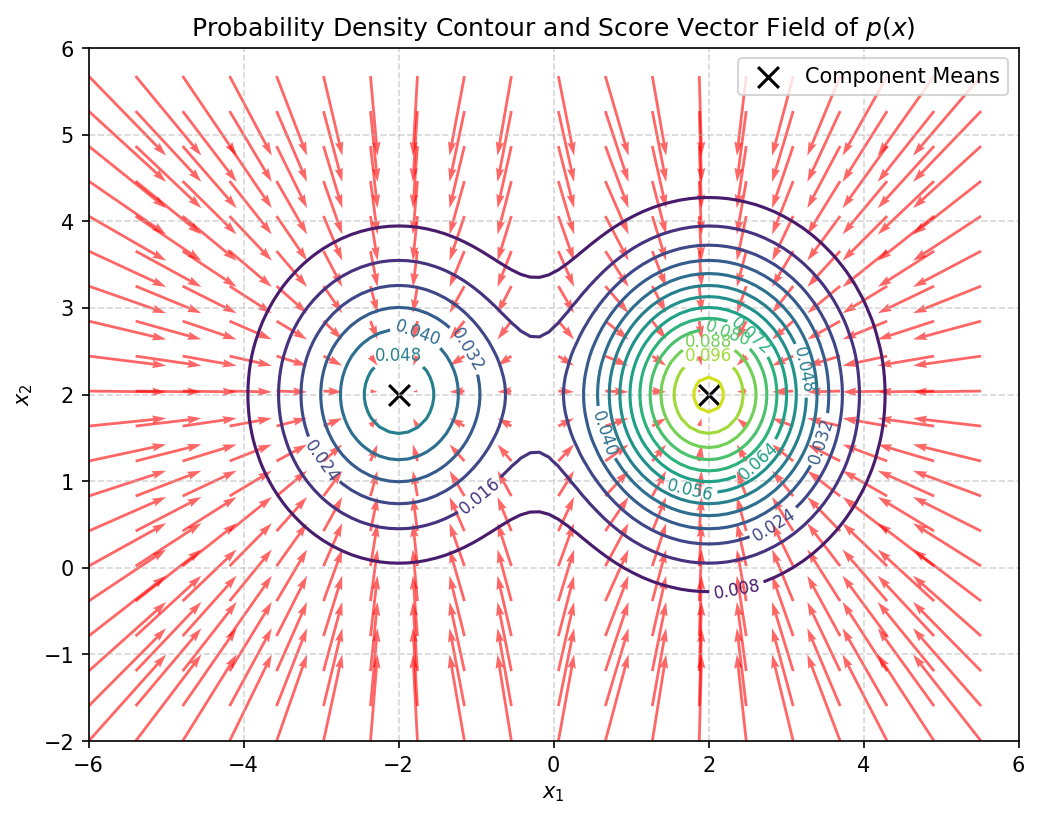
\includegraphics[width=0.70\textwidth]{problem4/plots/density_score_field.png}
    \caption{$p(x)$ の確率密度等高線と Score のベクトル場（赤矢印）。黒の $\times$ 印は各ガウス分布の平均値（ピーク）を示す。}
    \label{fig:density_score_field}
\end{figure}
\end{proofbox}

\subsection*{4.3}
\begin{note}
$p(x)$ に従う変数 $x$ に対し、
\[ y = x + \epsilon, \quad \epsilon \sim N (0, \tau^2 I) \]
と Gaussian Noise を加える。$p(y)$ の分布を混合 Gauss 分布の形として求めよ。\\
さらに、$\tau = 0.5, 1.5, 3.0$ の 3 通りについて、$p(y)$ の Score ベクトル場、Score の大きさ $\lVert \nabla_y \log p(y) \rVert$ をそれぞれプロットし、比較せよ。
\end{note}
\begin{proofbox}
ノイズを加えた後の確率変数 $y = x + \epsilon$ の確率密度関数 $p(y)$ は、確率密度の畳み込みで与えられる。
\[
p(y) = \int_{\mathbb{R}^2} p(x) N(y - x; 0, \tau^2 I) \, \mathrm{d}x = \sum_{i=1}^2 \pi_i \int_{\mathbb{R}^2} N(x; \mu_i, \sigma^2 I) N(y - x; 0, \tau^2 I) \, \mathrm{d}x
\]
独立なガウス分布の和の分布の再生性から、各ガウス成分 of 積分は $N(y; \mu_i, (\sigma^2 + \tau^2) I)$ となるため、
\[
p(y) = \frac{1}{3} N(y; \mu_1, (\sigma^2 + \tau^2) I) + \frac{2}{3} N(y; \mu_2, (\sigma^2 + \tau^2) I)
\]
が得られ、各成分の有効分散は $1 + \tau^2$ となる（$\sigma = 1$）。

$\tau = 0.5, 1.5, 3.0$ の3通りについて、Scoreのベクトル場（左）とScoreの大きさ $\lVert \nabla_y \log p(y) \rVert$（右）の比較プロットを図\ref{fig:noise_comparison}に示す。

\begin{figure}[H]
    \centering
    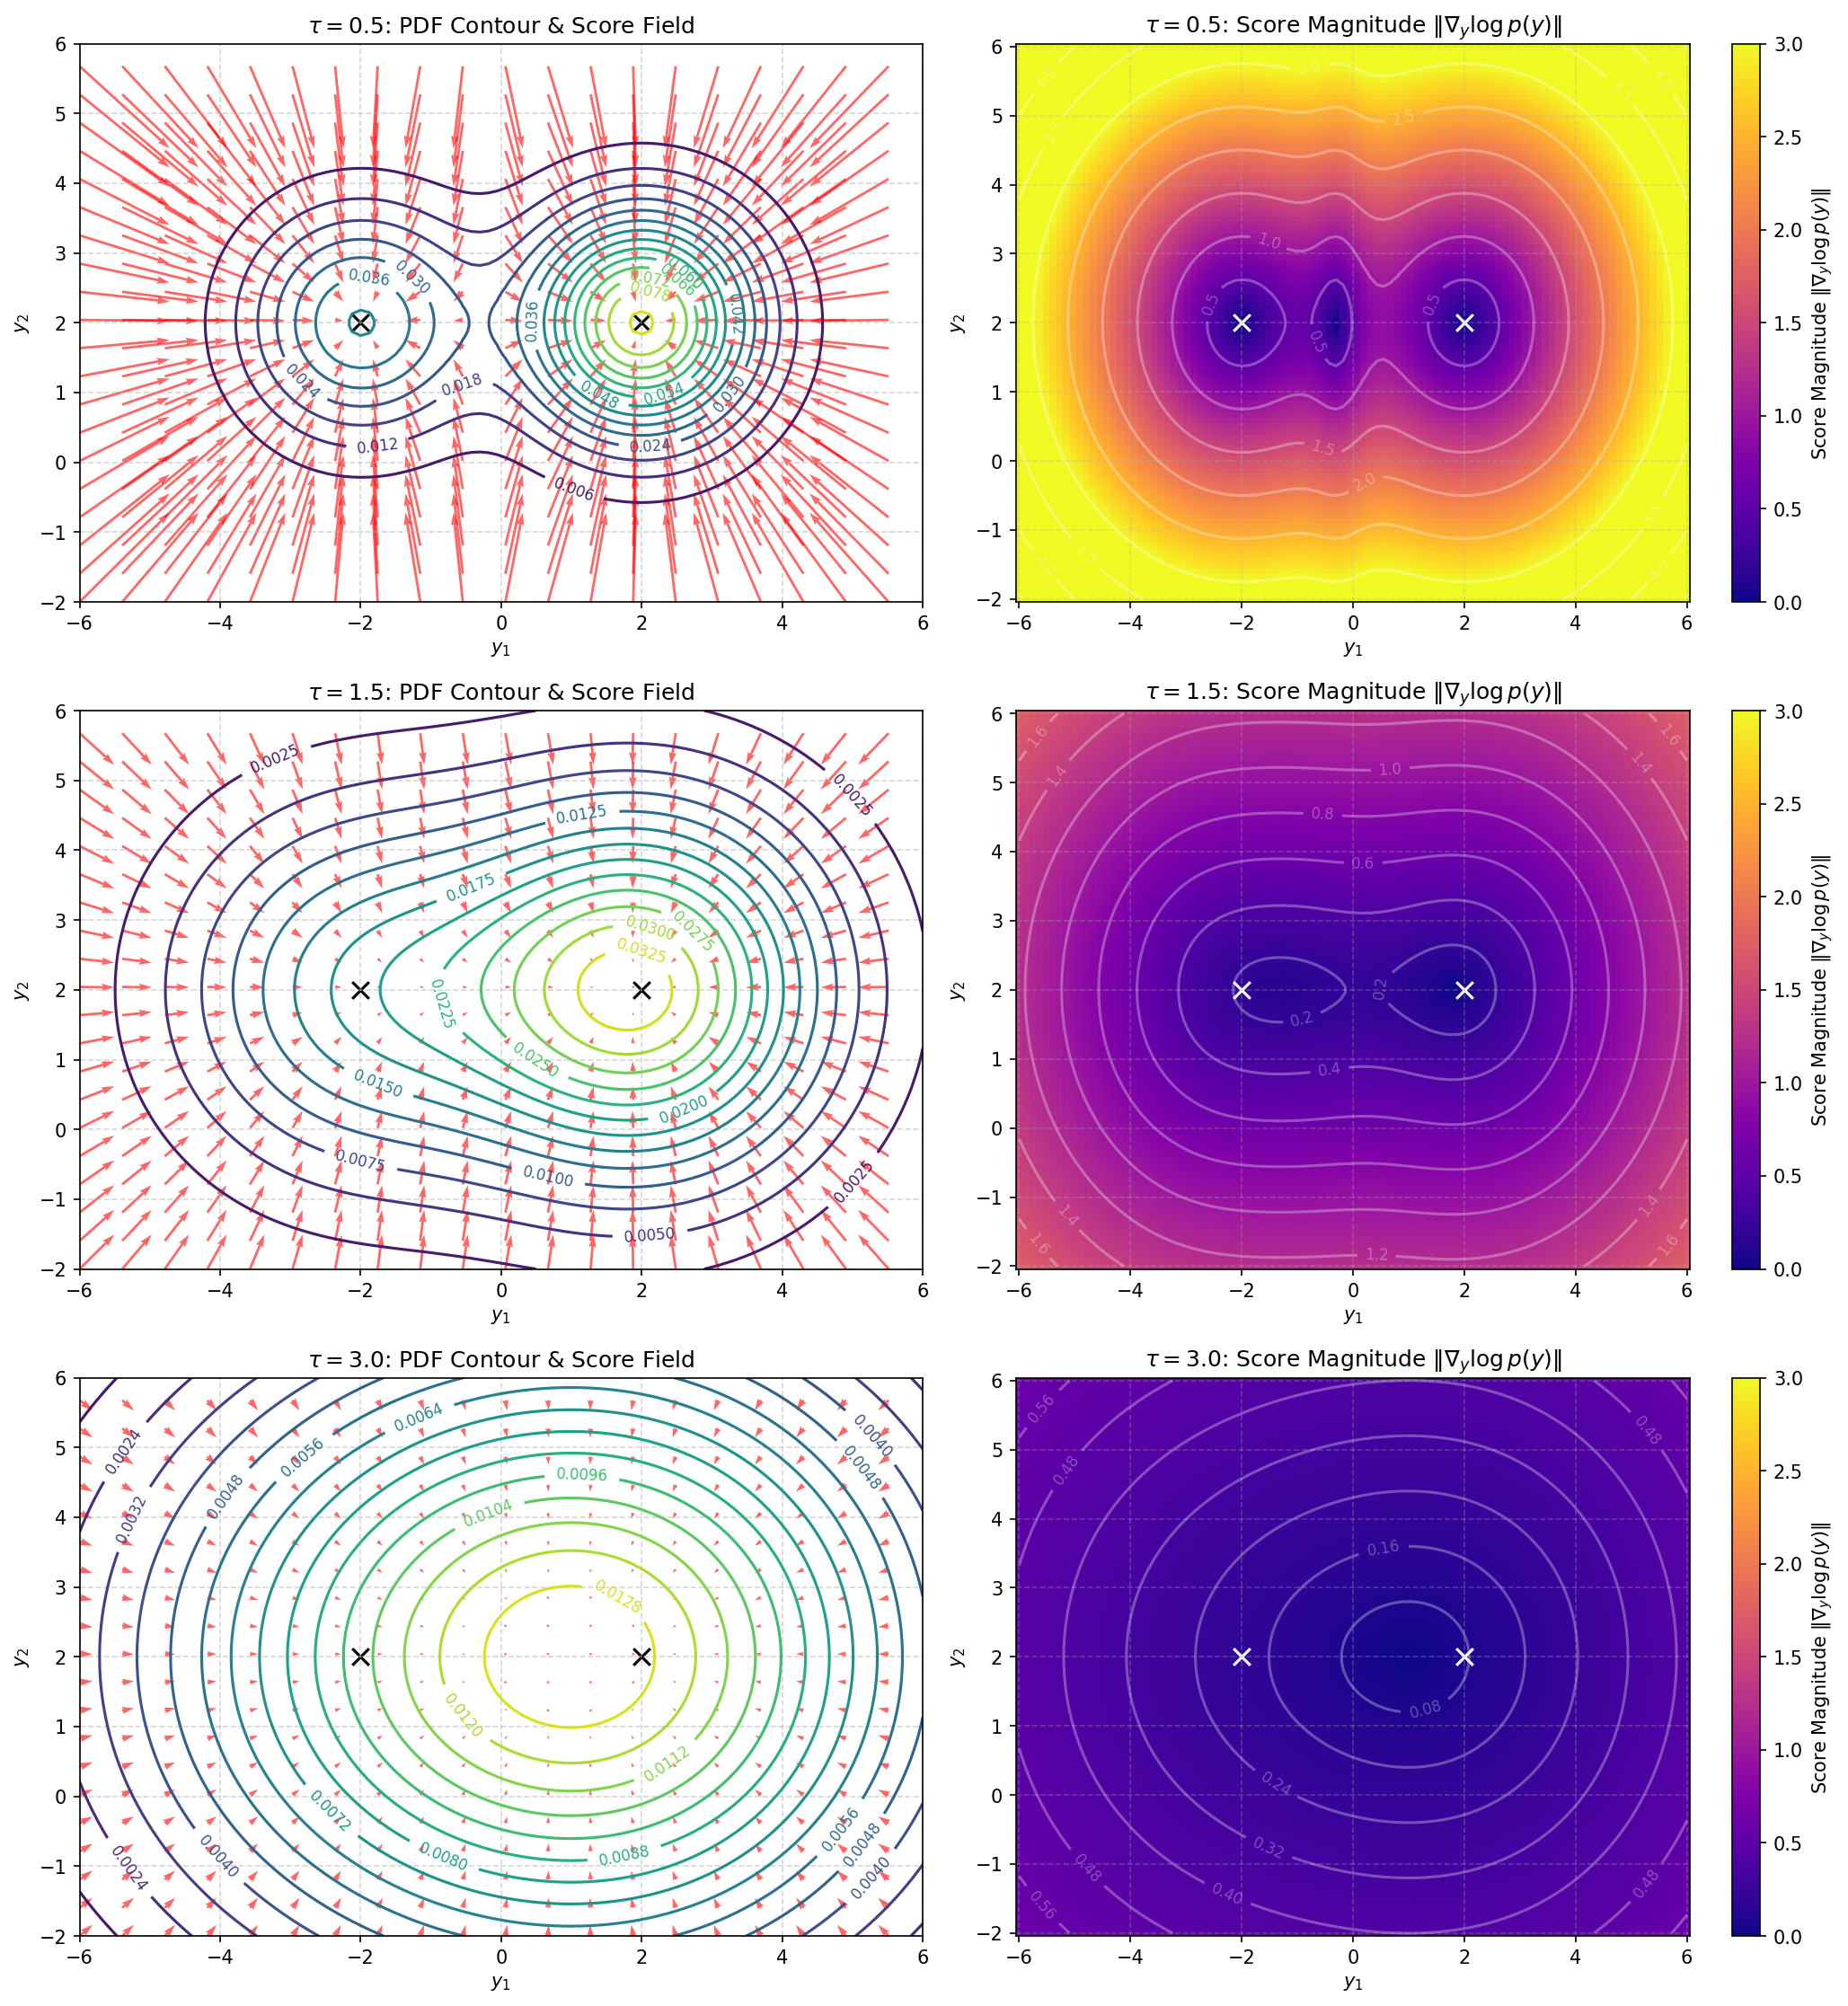
\includegraphics[width=0.95\textwidth]{problem4/plots/noise_comparison.png}
    \caption{各ノイズ強度 $\tau = 0.5, 1.5, 3.0$ における確率密度等高線と Score ベクトル場（左）、および Score の大きさ $\lVert \nabla_y \log p(y) \rVert$ のヒートマップ（右）。}
    \label{fig:noise_comparison}
\end{figure}
\end{proofbox}

\subsection*{4.4}
\begin{note}
上の実験で得られた結果について観察し、気づいたことを 3 つ以上挙げよ。考察はここでは書かず、次に書くこと。
\\
\end{note}
\begin{proofbox}
図\ref{fig:noise_comparison}から、以下の傾向が観察できる。

\begin{itemize}
    \item 確率密度の単峰化: $\tau = 0.5$ では2つの明確なピークがあるが、$\tau = 1.5$ では中央が平坦になり、$\tau = 3.0$ では完全に合流して非対称な（$y_1 > 0$ に偏った）単峰分布に変化する。
    \item Scoreベクトルの全体的な縮小と平坦化: $\tau$ が大きくなるにつれて有効分散が増大し、Scoreの大きさ（ヒートマップの明るさ）が全体的に著しく低下して、平坦な領域が広がる。
    \item 中間領域の挙動の解消: $\tau = 0.5$ のときは 2つのピークの中間（$y_1 = 0$ 付近）でScoreの向きが急激に反転（引き裂かれる挙動）しているが、$\tau$ が大きくなるとこれが解消され、全体の極大点へ向かう滑らかな流れに統合される。
\end{itemize}
\end{proofbox}

\subsection*{4.5}
\begin{note}
Noise が強くなるほど Score ベクトル場は平坦になることが予想される。この理由を説明せよ。また、そのことが Diffusion Model において異なる時刻ごとに Score を学習する理由とどのように関係しているか説明せよ。さらに、観察した他の事項についても、説明がつけば考察せよ。
\end{note}
\begin{proofbox}
ノイズ $\epsilon \sim N(0, \tau^2 I)$ が加わると有効分散は $\sigma^2 + \tau^2$ となる。単一ガウス分布のスコアが $-\frac{y-\mu}{s^2}$ でありその傾きが分散の逆数 $1/s^2$ に比例することから、ノイズ強度 $\tau$ が大きくなるほど各成分のスコア勾配は $1/(1+\tau^2) \to 0$ となり平坦化する。また、分散の拡大で2つのガウス分布の裾野が広く重なり合うため、互いに逆向きのベクトルが相殺し合い、ベクトル場全体が急速に平坦化する。

拡散モデルの生成プロセスでは、完全なノイズ状態から逆 Langevin 動力学によって段階的にノイズを低減させていくが、各ノイズ強度（時刻 $t$）ごとに異なるスコアを学習する理由は以下のように整理できる。
ノイズが大きい初期（$t$ が大きい）は確率密度が全空間に広がり、すべての点で安定した（平坦で緩やかな）スコアが定義される。この段階ではデータ空白域がないため、どこからスタートしても大まかにデータ領域へ誘導する大域的なマクロ構造を安定して学習できる。
その後、データが領域へ集まるにつれてノイズレベルを下げ、局所的で複雑なスコア（ミクロなディテール）を適用して精密に復元する。
もし単一のノイズ（$\tau \to 0$）のスコアのみでサンプリングしようとすると、データから遠い領域でスコアの推定が破綻して生成が失敗する（多様体仮説の課題）。そのため、時刻ごとにスコアを条件付けして学習させることが、安定した高精度な生成において不可欠である。
（スコアが平坦なノイズの大きい状態から学習を始めることが、実はニューラルネットが多様体の外で迷子になるのを防ぐ大域的な道標になっているのだと分かり、拡散モデルの設計の巧妙さに感心した。）
\end{proofbox}


\section*{[生成 AI]}

\subsection*{使用した AI}
\begin{note}
本課題においてどの生成 AI を使用したか、モデルを含めて書け。なぜその AI を選んだか、理由もあれば書くこと。
\end{note}
\begin{proofbox}
本課題では、Google DeepMindの開発した \textbf{Gemini 3.5 Flash} (Medium / Flashモデル) を使用した。このモデルを選択した理由は、マルチファイルコンテキストの処理能力が高く、LaTeXの数式コードやPythonの実行スクリプト等の複数ファイルを正確に把握しながら、高速かつ的確な応答が得られるためである。
\end{proofbox}

\subsection*{工夫}
\begin{note}
各問題に対して AI を使った時の会話ログの共有リンクを載せよ。また、その会話で行った工夫や意識した点があれば書け (ex. AI に自分の考えを先に説明した、AI の回答を検証した)。共有リンクを作成すると公開情報になるため、本名や学籍番号などの個人情報は会話に入れないよう注意すること。
\end{note}
\begin{proofbox}
各問題の解答作成時にAIと対話したセッションの会話ログ、および本レポートに付随する理論・数式解説ドキュメントは、個人情報を除外した形でマークダウンファイルとして保存し、以下の一般公開GitHubリポジトリにアップロードした。
\begin{itemize}
    \item リポジトリURL: \href{https://github.com/KokinCho/4S_physics_public/tree/main/\%E6\%A9\%9F\%E6\%A2\%B0\%E5%AD\%A6\%E7%BF%92%E6%A6%82%E8%AB%96/\%E5%BE%8C%E5%8D%8A%E3%83%AC%E3%83%9D%E3%83%BC%E3%83%88}{\texttt{https://github.com/KokinCho/4S\_physics\_public/tree/main/機械学習概論/後半レポート}}
    \item 会話ログファイル: 
    \begin{itemize}
        \item \texttt{conversation\_with\_Gemini\_3\_5\_Flash\_1(Transcribing Exam Questions to LaTeX).md} (後半レポートの問題文書き起こし、およびGPRとMLPの比較（問題1）のシミュレーション実装と考察の対話)
        \item \texttt{conversation\_with\_Gemini\_3\_5\_Flash\_2(Solving VAE Report Problems).md} (変分オートエンコーダ（VAE）におけるELBOの数学的分解とKLダイバージェンスの解析的計算（問題3）の対話)
    \end{itemize}
    \item 副生成された学習用の数式・理論解説ファイル: 
    \begin{itemize}
        \item \texttt{scratch/math\_explanation\_gp\_mlp.md} (ガウス過程回帰とMLPの予測波形の比較に関する理論解説)
        \item \texttt{scratch/math\_explanation\_gp\_mlp\_nature.md} (GPRの条件付き期待値とMLPの非線形写像点推定に関する詳細と授業スライド参照先)
        \item \texttt{scratch/math\_explanation\_gp\_waviness.md} (GPRの予測信頼区間におけるうねりと一様性の統計的要因分析)
        \item \texttt{scratch/math\_explanation\_em\_algorithm.md} (混合正規分布におけるEMアルゴリズムの直感的解釈とE/Mステップの意味)
        \item \texttt{scratch/math\_explanation\_em\_general.md} (EMアルゴリズムの一般形における対数尤度最大化の困難性とLog-of-Sum問題の解説)
        \item \texttt{scratch/math\_explanation\_elbo.md} (尤度下界（ELBO）の分解式の意味、PRMLの床と天井の関係図、および日本人身長を例とした各分布の具体化)
        \item \texttt{scratch/math\_explanation\_autoencoder.md} (オートエンコーダの構造と線形時における主成分分析（PCA）との数学的等価性の証明)
        \item \texttt{scratch/math\_explanation\_vae\_intro.md} (VAEの設計思想、標準正規分布からのサンプリング、およびデコーダが確率分布パラメータを出力する意図)
        \item \texttt{scratch/math\_explanation\_vae\_idea.md} (VAEにおけるエンコーダ/デコーダの双対最適化、不可能積分の回避、および誤差逆伝播法との親和性)
        \item \texttt{scratch/math\_explanation\_vae.md} (VAEのELBO最大化とKLダイバージェンス展開に関する数式証明)
    \end{itemize}
\end{itemize}

AIを利用するにあたり意識した工夫は以下の通り。第一に、理論的な理解を曖昧にしたまま答えを生成させるのではなく、スライドの疑問点について「EMアルゴリズムにおける周辺尤度の Log-of-Sum の壁」や「VAEにおけるサンプリングの確率的ゆとり」など、理論の行間を丁寧に質問・言語化させながら進めた。第二に、AIが生成した数式やコードを鵜呑みにせず、GPRの信頼区間が $n \to \infty$ で $0$ に収束するような不自然な解説に対して「観測ノイズがあるためノイズ幅に漸近するはずだ」と自ら論理的矛盾を指摘し、数学的に厳密な表現へと修正させた。第三に、自身の自学自習用に、数式展開の背景にある物理的・統計的意味を通しの具体例（身長と性別）を交えて解説書として別途まとめさせることで、レポート執筆と自己学習を並行させた。
\end{proofbox}

\subsection*{感想}
\begin{note}
AI を利用したことで理解が深まった点、逆に AI では解決できなかった点があれば書け。
\end{note}
\begin{proofbox}
\textbf{【理解が深まった点】} \\
ガウス過程回帰における予測分布の導出や、MLPがデータ不足でうねる原因について、授業スライドとコードの両面から検証したことで、数理的な理解が飛躍的に深まった。また、EMアルゴリズムからVAEへと至る「事後分布の不可能積分を回避するための近似ネットワークの導入」という設計思想の繋がりや、オートエンコーダが線形極限でPCAと等価になるという美しい数学的性質、さらにELBOの変形におけるKLダイバージェンスが意味する「天井と床の隙間」の直感的理解など、スライドだけでは見落としがちだった数理の行間が、AIとの対話と副生成した数理ドキュメント群のトレースによって深く腹落ちした。

\textbf{【解決できなかった点】} \\
LaTeXの日本語コンパイル環境（特に \texttt{latexmk} から \texttt{pdflatex} への暗黙的なエンジン切り替えやフォントエンコーディングの設定）の違いにより、日本語のマルチバイト文字がUnicodeエラーを引き起こす問題について、AIは当初のコンパイルエラーに対して適切な uplatex コマンドでの解決策を自立的に提案できず、手動でコマンドの切り替え（\texttt{uplatex} + \texttt{dvipdfmx} の明示）を行う必要があった。ローカルのビルドツールチェーンの依存関係の解消には、AIの提案に頼るだけでなく、人間側の環境調整が必要であることを実感した。
\end{proofbox}
\begin{thebibliography}{10}
    %(本)著者名. 書名. 出版社, 出版年.
    %(雑誌論文)著者名. 論文名. 誌名. 出版年, 巻数, 号数, p.始め-終わり.
    %(web)著者名. “ページ名”. サイト名. 更新日. 入手先URL, (閲覧日).
    \bibitem[1]{kabashima2025} 樺島祥介. “機械学習概論” 講義資料 (2025年度). 東京大学大学院理学系研究科.
\end{thebibliography}

\end{document}